\documentclass[a4paper,11pt]{article}

% Ces 2 là doivent être les 2 premiers
\usepackage[utf8]{inputenc}
\usepackage[T1]{fontenc}

\usepackage[a4paper]{geometry}

\usepackage{amsfonts}
\usepackage{amsmath}
\usepackage{mathtools}
% \usepackage{bbm}
\usepackage{graphicx}
% \usepackage{tikz}
% \usepackage{mdwlist}

% Babel est après tous les paquets sauf: eurosym, varioref, floatrow,
% caption, subcaption, listings, datetime2
\usepackage[french]{babel}

% \usepackage{subcaption}
% \usepackage{listings}
% \lstset{ %
%   language=Fortran,
%   basicstyle=\footnotesize,           % the size of the fonts that are used for the code
%   numbers=left,                   % where to put the line-numbers
%   numberstyle=\tiny\color{gray},  % the style that is used for the line-numbers
%   stepnumber=5,                   % the step between two line-numbers. If it's 1, each line 
%                                   % will be numbered
%   numbersep=5pt,                  % how far the line-numbers are from the code
%   frame=single,                   % adds a frame around the code
%   breaklines=true,                % sets automatic line breaking
%   breakatwhitespace=false,        % sets if automatic breaks should only happen at whitespace
%   title=\lstname,                   % show the filename of files included with \lstinputlisting;
%   }

% hyperref est en dernier, sauf pour hypcap, bookmark, glossaries,
% cleverref, autonum
\usepackage{hyperref}

\geometry{vmargin=2cm,hmargin=2.5cm,nohead}

\DeclareMathOperator{\diag}{diag}
\DeclareMathOperator{\dv}{div}
\DeclareMathOperator{\tr}{tr}
\DeclareMathOperator{\Id}{Id}
\DeclareMathOperator{\atan}{atant}
% \DeclareMathOperator{\Re}{Re}
% \DeclareMathOperator{\Im}{Im}

\def \kk     {{\mathbb K}} 
\def \nn     {{\mathbb N}} 
\def \cc     {{\mathbb C}} 
\def \rr     {{\mathbb R}} 
\def \zz     {{\mathbb Z}}

\def \f      {{\mathbf f}}
\def \g      {{\mathbf g}}
\def \u      {{\mathbf u}}
\def \v      {{\mathbf v}}

\def \P {\text{P}}
\def \Q {\text{Q}}
\def \b {\text{b}}

\def \o      {{\Omega}}

\def \un     {{\mathbf 1}}

\newcommand{\abs}[1]{\lvert#1\rvert}

\newcounter{exerc}[section] %  Compteur du numéro d'exercice, 
                            % remis à zéro par section
\newenvironment{exercice}[1]{
  \addtocounter{exerc}{1}
  \paragraph{\bf Exercice~\arabic{exerc} : #1}\hfill\mbox{}\par}{}

\newenvironment{questions}{\begin{enumerate}}{\end{enumerate}}

\begin{document}

\begin{center}
  \parbox{0.8\linewidth}{
    \begin{center}\large
      \emph{Master MAS, parcours MNCHP}\\ Méthodes numériques pour les
      écoulements incompressibles \\[2ex]
      \emph{AN312}\\ Simulation numérique par éléments finis avancés \\
      [2ex] 2018/2019
    \end{center}%
  }
\end{center}

\subsection*{FreeFem++}

\begin{itemize}
\item Page web~: \url{http://www.freefem.org/ff++/}
\item Documentation~:
  \url{http://www.freefem.org/ff++/ftp/freefem++doc.pdf}
\item Principe~: FreeFem++ est un interpréteur de script (comme matlab,
  python, scilab...) dédié à la résolution approchée par éléments finis
  de problèmes mis sous forme variationnelle. C'est un idiome de C++.
\item On écrit donc des fichiers contenant des commandes, par exemple
  {\tt exple.edp}, que l'on exécute dans un terminal X en utilisant la
  commande suivante~:
  \begin{flushleft}
    \tt $\ldots$\$ FreeFem++ exple.edp 
  \end{flushleft}
  L'exemple fournit (fichier {\tt exple.edp}) construit un maillage du
  carré $(0,1)\times(0,1)$ ayant 10 éléments par côté représenté
  ci-dessous.
  \begin{center}
    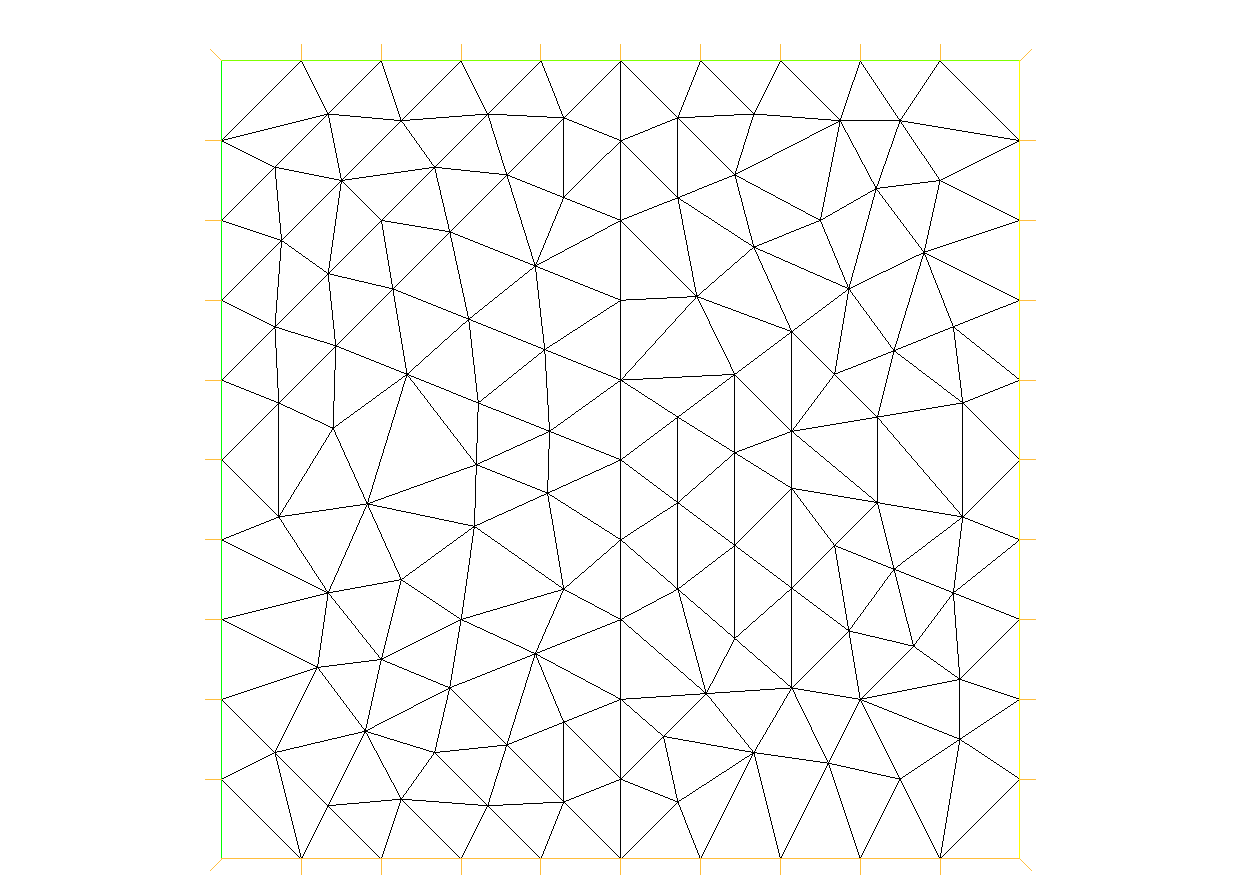
\includegraphics[width=0.6\linewidth]{exple.pdf}
  \end{center}
\item Quelques éditeurs de fichiers supportent une colorisation
  syntaxique pour FreeFem++: atom, emacs, vi...
  \begin{itemize}
  \item Avec emacs: \url{https://github.com/holomorph/emacs-freefem} or
    \url{https://github.com/rrgalvan/freefem-mode}
  \item Avec Atom: \url{https://atom.io/packages/language-freefem}
  \end{itemize}
  % \begin{itemize}
  % \item {\tt nedit}, en éxécutant une seule fois {\tt \$ nedit -import
  %     edp.nedit};
  % \item {\tt emacs}, grâce au mode d'édition {\tt ff++-mode-0.2.el},
  %   voir \\\url{http://softwarelibre.uca.es/node/946}.
  % \end{itemize}
\item Il existe aussi un environnement de développement intégré (IDE)
  pour FreeFem++, voir
  \url{https://www.ljll.math.upmc.fr/lehyaric/ffcs/index.htm}. 
\end{itemize}

% \subsection*{Bibliothèques d'algèbre linéaire}

% \begin{itemize}
% \item BLAS (\url{http://www.netlib.org/blas/}) est en général installé
%   sur tout système de calcul scientifique. C'est une bibliothèque aui
%   implémente des opérations entre matrices et vecteurs. Sur chaque
%   système, il existe des versions optimisées. Par exemple Intel
%   fournit une implémentation de BLAS dans la bibliothèque mkl,
%   \url{https://software.intel.com/en-us/intel-mkl}.
% \item UMFPACK est une bibliothèque qui fait partie de la suite
%   logicielle {\tt Suitesparse}
%   (\url{http://faculty.cse.tamu.edu/davis/suitesparse.html}), utilisée
%   en particuler dans {\tt Matlab} (fonction \og $\backslash$
%   \fg). C'est une bibliothèque de résolution des systèmes linéaires
%   creux par une méthode directe (décomposition LU). Elle utilise un
%   système de stockage CSC (Compressed Sparse Column) des matrices.
% \end{itemize}

% \smallskip 
% \centerline{\rule{0.75\linewidth}{1pt}}
% \medskip

\begin{exercice}{Problème de Laplace}

  \begin{equation}
    \label{eq:laplace}
    -\dv(a(x) \nabla u) = f \quad\text{dans }\o,\quad u=g\quad\text{sur }\partial\o.
  \end{equation}
  où $\xi^T a(x) \xi \ge a_0 |\xi|^2$ (pour tout $\xi\in\rr^2$) avec
  $a_0>0$, et $x\mapsto a(x)$ est une fonction mesurable et majorée.

  Le fichier {\tt laplace.edp} va nous servir de modèle. Il permet de
  faire un calcul d'erreur de convergence pour un problème du type
  \eqref{eq:laplace} avec $a(x) = 1$, dont on connaît la solution
  exacte. Ici, on a choisit la fonction $u(x,y) = x(1-x)*y(1-y)$ qui est
  telle que $u(x,y) = 0$ sur $\partial\o$. Le script permet de répéter
  le calcul sur une famille de maillage du plus en plus fins, de telle
  sorte que l'on peut étudier la convergence et l'erreur commise par le
  schéma.

  Prenez le temps de bien détailler et comprendre le fonctionnement de
  ce script. Exécutez-le, éventuellement en faisant des petites
  modifications (par exemple de l'élement P1-Lagrange choisit ici, de la
  finesse des maillages...).

  Attention, il faut créer le répertoire {\tt output} dans lequel le
  script écrit ses résultats avant d'exécuter le script: {\tt \$ mkdir
    output}, puis {\tt \$ Freefem++ laplace.edp}.

  Le script gnuplot fournit ({\tt plot\_laplace.gp}) permet de tracer le
  graphe de l'erreur en norme $L^2$ sur la solution $u$ (en exécutant
  {\tt \$ gnuplot plot\_laplace.gp}).
  \begin{figure}[hbp!]
    \centering
    \label{fig:1}
    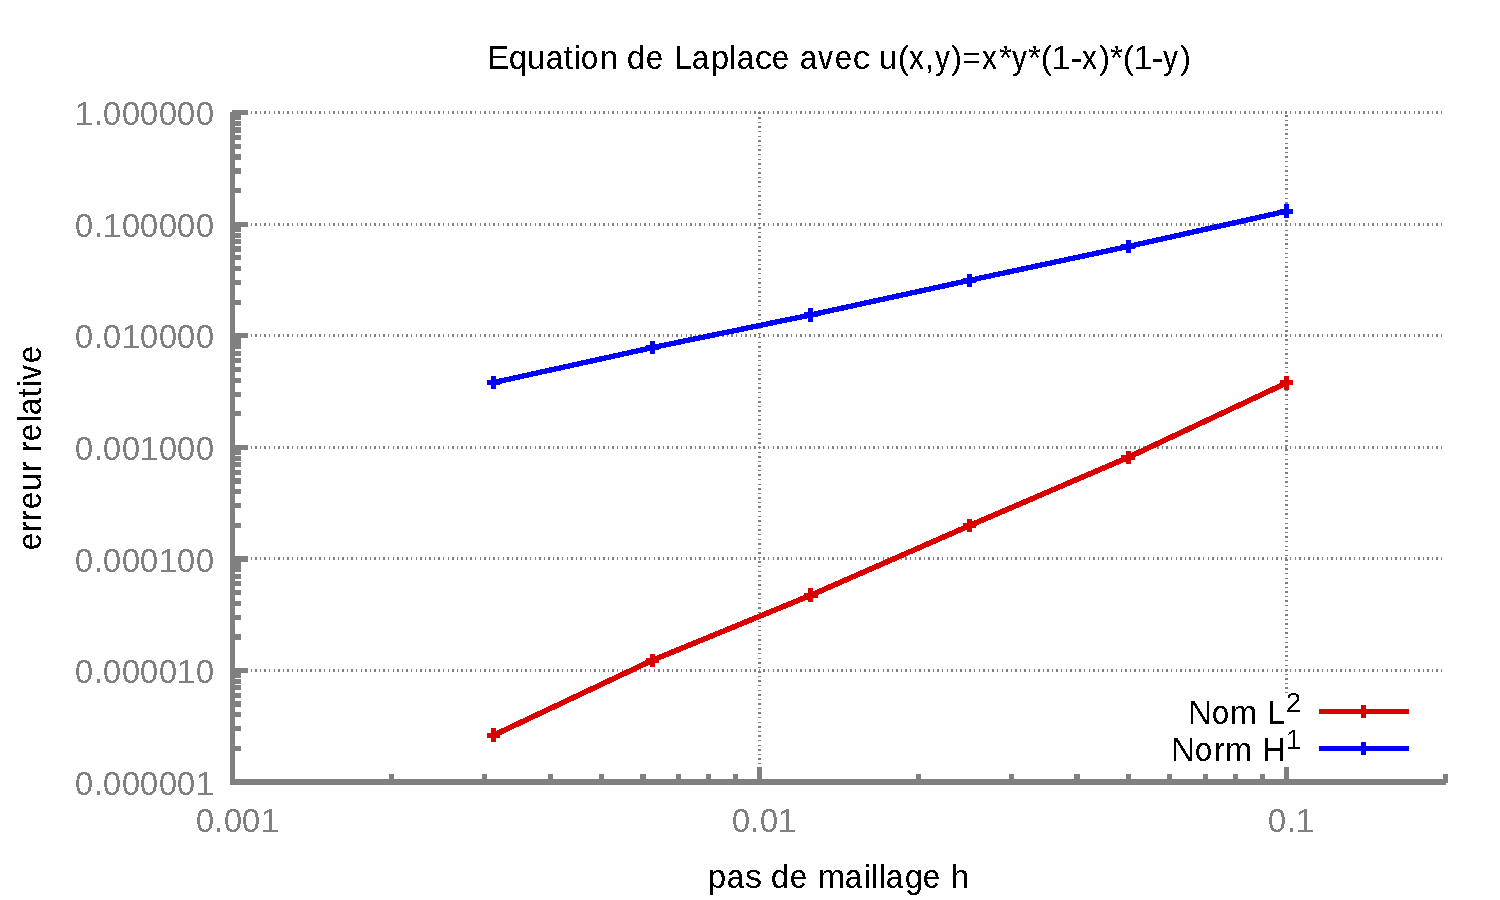
\includegraphics[width=0.45\linewidth]{output/laplace_errors_umfpack.pdf}
    \hskip 1em
    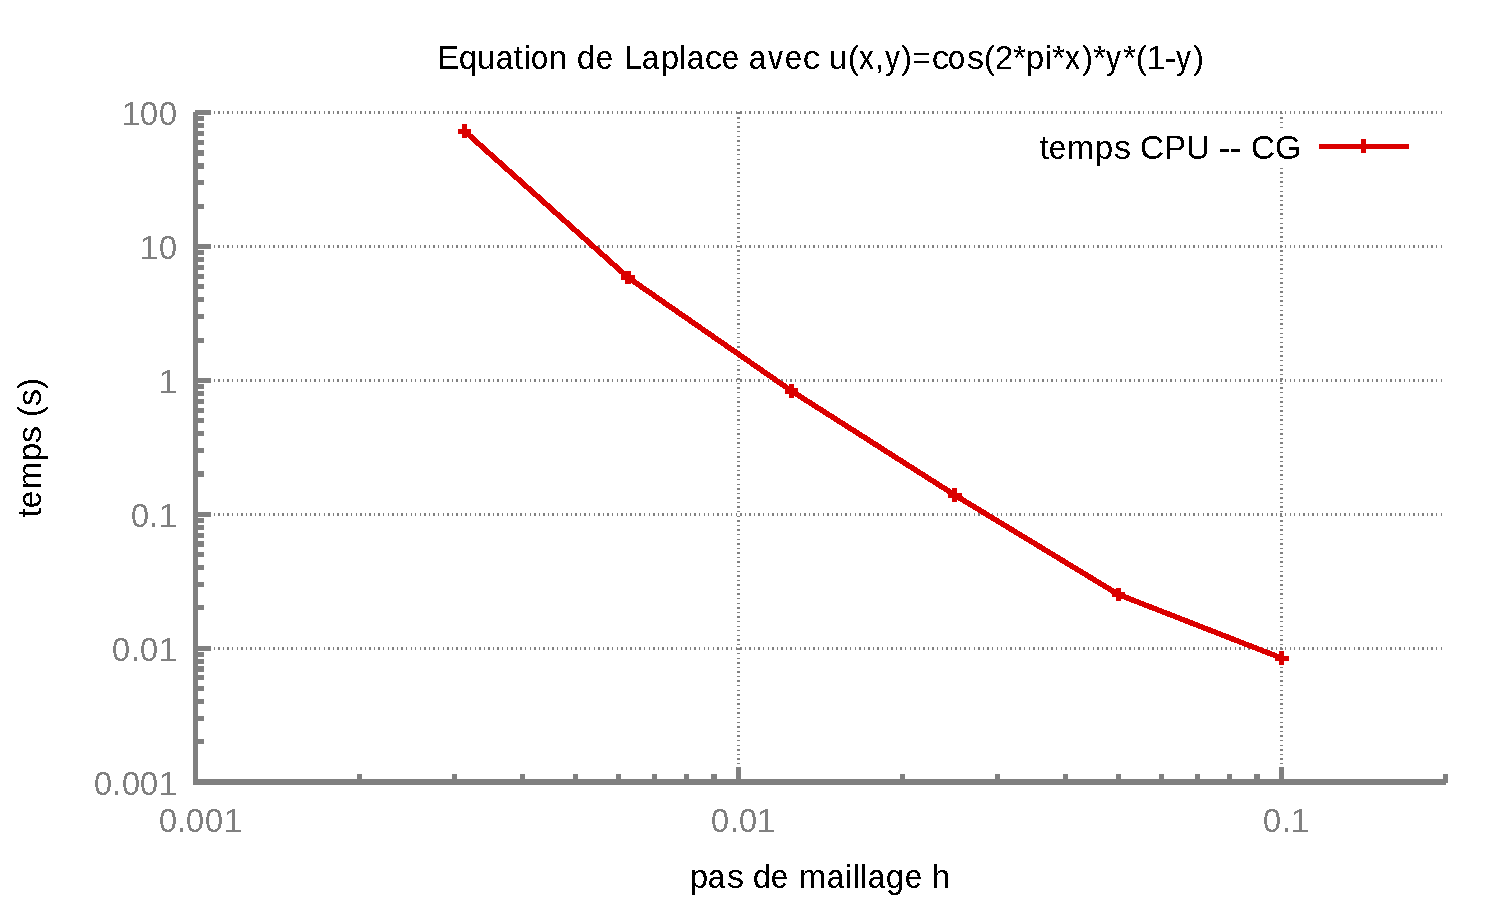
\includegraphics[width=0.45\linewidth]{output/laplace_cpu.pdf}
    \caption{Erreurs et temps CPU pour le problème de Laplace}
  \end{figure}

  \begin{enumerate}
    
  \item Programmer le calcul de l'erreur en norme $H^1$, définie par
    $E_{H^1} = \left( \int_\o \left| \nabla u - \nabla u_h \right|^2 dx
    \right)^{1/2}$. Puis rajouter le graphe de cette erreur sur le
    graphique précédent (obtenir le graphique de la
    figure~\ref{fig:1}). À partir de vos connaissance sur les éléments
    finis, que pouvez vous dire de ces graphes de convergence ?

    Donner les tableaux de valeurs $\min(u_h(x))$, $\max(u_h(x))$, et
    $\min(u(x))$, $\max(u(x))$. Pour certaines applications, il est
    important de conserver ces $\min$ et $\max$. Que se passe-t-il pour
    notre problème ?

  \item Reproduire l'analyse pour la fonction solution $u(x,y) = x+y$
    (attention, il faut modifier le second membre $f$ et la valeur au
    bord $g$). Vérifier avec cette solution que les élements finis P1
    sont exacts quel que soit le maillage utilisé.

  \item Reproduire l'analyse pour la fonction solution
    $u(x,y) = \cos(2\pi x)y(1-y)$ en calculant le second membre associé, et en
    utilisant les conditions aux limites mêlées~: $u = 0$ sur $\{y=0\}$ et
    $\{y=1\}$, et $\nabla u\cdot n = 0$ sur $\{x=0\}$ et $\{x=1\}$.

  \item On fixe le maillage le plus fin possible pour résoudre le
    système linéaire en un temps raisonable avec Umfpack. Pour ce
    maillage, évaluer l'erreur commise pas la résolution par une les
    méthodes itératives CG et GMRES en variant la tolérance souhaitée de
    $10^{-1}$ à $10^{-13}$. Comparer aussi le temps de calcul par
    rapport au temps mis pour la méthode LU de Umfpack.

  \item On fixe maintenant la tolérance du solveur CG (puis GMRES) à
    $10^{-10}$. Comparer les temps de calcul de ces deux méthodes
    itératives avec celle de la méthode directe pour la suite de
    maillage utilisée aux questions précédentes.

  \item On prend maintenant un cas fortement anisotrope,
    $a(x) = \diag(1.,10^r)$, avec des conditions de Dirichlet homogène
    et le second membre $f := 4\pi^2(1+10^r) \sin(2\pi x)\sin(2\pi
    y)$. Dans ce cas, la solution exacte est
    $u = \sin(2\pi x)\sin(2\pi y)$. Étudier le schéma numérique pour ce
    cas test avec quelques valeurs de $r$, par exemple $r=1,3,6$.

    % Cas tests anisotropes, coefficients discontinus... à écrire.
    
    % \item On pourra aussi programmer une version tri-dimensionnelle et refaire ces
  %   mêmes tests, ou encore tester des éléments finis d'ordre plus élevé (P2,
  %   P3...), et observer l'amélioration de la convergence.

  \end{enumerate}

\end{exercice}

\end{document}



